\documentclass[12pt]{article}

%%%  PACKAGES
\usepackage[utf8]{inputenc}
\usepackage{geometry}
\usepackage[frenchb]{babel}
\usepackage[T1]{fontenc}
\usepackage{array}           % for better arrays (eg matrices) in maths
\usepackage{subfig}			% make it possible to include more than one captioned figure/table in a single float
\usepackage{paralist}		% very flexible & customisable lists (eg. enumerate/itemize, etc.)
\usepackage{verbatim} 		% adds environment for commenting out blocks of text & for better verbatim
\usepackage{graphicx}		% Inclusion d'images-> \noindent\includegraphics[width=400px]{name}
\graphicspath{{images/}}		% le chemin ou aller chercher les graphics
\usepackage{listings}		% package for code listing
\usepackage{color}			% package to use color
\usepackage{hyperref}        % pour les liens cliquables (url, etc....)

%%%  PAGE DIMENSIONS
\geometry{a4paper} % or letterpaper (US) or a5paper or....
\geometry{a4paper, left=20mm, right=20mm, bottom=25mm, top=25mm}
\setlength{\parskip}{0.5em} % Espace entre les paragraphes

%%% USER COLORS
\definecolor{darkGreen}{RGB}{0,0.6,0}
\definecolor{gray}{RGB}{0.5,0.5,0.5}
\definecolor{mauve}{RGB}{0.58,0,0.82}
\definecolor{pblue}{rgb}{0.13,0.13,1}
\definecolor{pgreen}{rgb}{0,0.5,0}
\definecolor{pred}{rgb}{0.9,0,0}
\definecolor{pgrey}{rgb}{0.46,0.45,0.48}
\definecolor{red}{rgb}{1,0,0}
\definecolor{green}{rgb}{0,1,0}

%%% CODE STYLE (\lstinputlisting{stcFile.cpp} ou \begin{lstlisting} et \end{lstlisting}

%%% JAVA STYLE
\lstdefinestyle{Java}
{
  language=Java,
  inputencoding=utf8,
  frame=single,
  showspaces=false,
  showtabs=false,
  breaklines=true,
  showstringspaces=false,
  breakatwhitespace=true,
  commentstyle=\color{pgreen},
  keywordstyle=\color{pblue},
  stringstyle=\color{pred},
  basicstyle=\fontsize{9}{11}\ttfamily,
  numbers=left,
  numbersep=5px,
  numberstyle=\tiny\color{pgrey},
  stepnumber=1,
  tabsize=2,
}

%%% C++ STYLE
\lstdefinestyle{c++}
{
  language=C++,
  inputencoding=utf8,
  showtabs=false,
  breaklines=true,
  breakatwhitespace=true,
  stepnumber=1,
  basicstyle=\fontsize{9}{11}\ttfamily,
  commentstyle=\color{mygray},
  frame=single,
  numbers=left,
  numbersep=5px,
  numberstyle=\tiny\color{mygray},
  keywordstyle=\color{pblue},
  showspaces=false,
  showstringspaces=false,
  stringstyle=\color{myorange},
  tabsize=2
}

%%% XML Style
\lstdefinestyle{XML}
{
  inputencoding=utf8,
  language=XML,
  frame=lines,
  showspaces=false,
  showtabs=false,
  breaklines=true,
  showstringspaces=false,
  breakatwhitespace=true,
  commentstyle=\color{pgreen},
  keywordstyle=\color{pblue},
  stringstyle=\color{pred},
  basicstyle=\fontsize{9}{11}\ttfamily,
  numbers=left,
  numbersep=5px,
  numberstyle=\tiny\color{pgrey},
  stepnumber=1,
  tabsize=2
}

%%% JSON Style
\lstdefinestyle{JSON}
{
  inputencoding=utf8,
  frame=lines,
  showspaces=false,
  showtabs=false,
  breaklines=true,
  showstringspaces=false,
  breakatwhitespace=true,
  comment=[l]{:},
  commentstyle=\color{black},
  keywordstyle=\color{pblue},
  string=[s]{"}{"},
  stringstyle=\color{pblue},
  basicstyle=\fontsize{9}{11}\ttfamily,
  numbers=left,
  numbersep=5px,
  numberstyle=\tiny\color{pgrey},
  stepnumber=1,
  tabsize=2
}

%%% PHP Style
\lstdefinestyle{PHP}
{
  language=PHP,
  inputencoding=utf8,
  frame=lines,
  showspaces=false,
  showtabs=false,
  breaklines=true,
  showstringspaces=false,
  breakatwhitespace=true,
  comment=[l]{:},
  commentstyle=\color{black},
  keywordstyle=\color{pblue},
  string=[s]{"}{"},
  stringstyle=\color{pblue},
  basicstyle=\fontsize{9}{11}\ttfamily,
  numbers=left,
  numbersep=5px,
  numberstyle=\tiny\color{pgrey},
  stepnumber=1,
  tabsize=2
}

% Setup pour les liens
\hypersetup{
    bookmarks=true,         % show bookmarks bar?
    unicode=false,          % non-Latin characters in Acrobat’s bookmarks
    pdftoolbar=true,        % show Acrobat’s toolbar?
    pdfmenubar=true,        % show Acrobat’s menu?
    pdffitwindow=false,     % window fit to page when opened
    pdfstartview={FitH},    % fits the width of the page to the window
    pdftitle={My title},    % title
    pdfauthor={Author},     % author
    pdfnewwindow=true,      % links in new PDF window
    colorlinks=true,        % false: boxed links; true: colored links
    linkcolor=black,        % color of internal links (change box color with linkbordercolor)
    citecolor=green,        % color of links to bibliography
    filecolor=magenta,      % color of file links
    urlcolor=blue,          % color of external links
}

%%%  HEADERS & FOOTERS
\usepackage{fancyhdr}                   % This should be set AFTER setting up the page geometry
\pagestyle{fancy}                       % options: empty, plain , fancy
\renewcommand{\headrulewidth}{1pt}      % customise the layout...
\renewcommand{\footrulewidth}{1pt}
\lhead{
\includegraphics[width=50px]{logoheig2}}\chead{}\rhead{Projet IOT}
\lfoot{T. Besseau, M. Chatelan, L. Chauffoureaux, E. Schmid}\cfoot{}\rfoot{\thepage}

%%% SETTINGS %%%
\setlength\parindent{0pt} 		% Taille de l'indentation
\headsep =40pt
\setcounter{tocdepth}{2}

%%% TITLE
\title{
  \vspace{-0.5cm}
  \huge{Projet IOT} \\
  \vspace{5mm}
  \Large{Analyse de menaces} \\
  \vspace{2.5cm}
  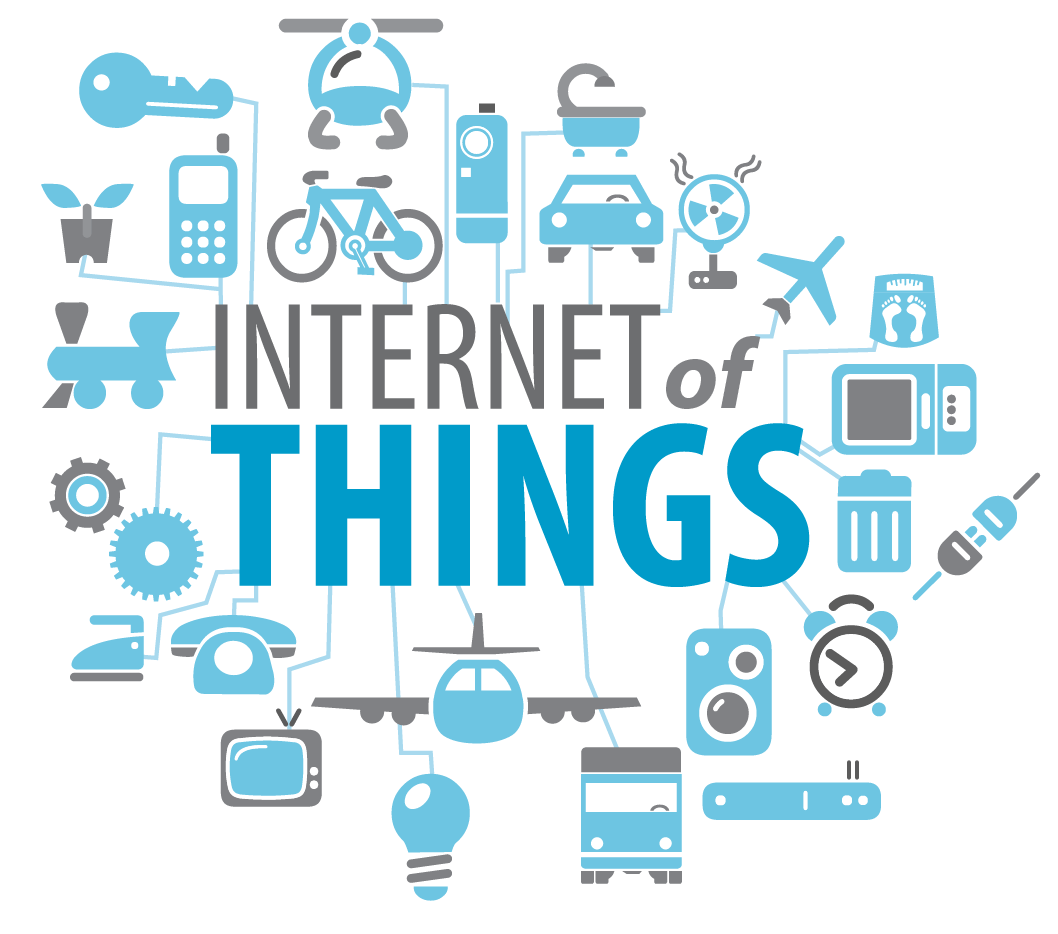
\includegraphics[width=.7\textwidth]{logo}
  \vspace{3cm}
}

\author{Thibaud Besseau, Matthieu Chatelan, Lara Chauffoureaux, Emmanuel Schmid}
\date{\today}

\begin{document}

\maketitle
\thispagestyle{empty}
\clearpage
\tableofcontents
\clearpage
\listoffigures
\clearpage
\headsep=20pt

\section{Introduction}
Ce document a pour but la sécurisation du projet élaboré dans le cadre du cours IoT dispensé à la HEIG-VD. Ce dernier est un ....... . Dans ce document, les exigences du projet en général seront décrites ainsi que les biens nécessitant une protection contre tout type de menaces ou tout scénarios d'attaque ainsi que les contre-mesures associées. Toutes les technologies utilisées pour ce projet ont été prises en compte.

\subsection{Equipes}
Lors de ce projet, nous avons créé 5 groupes distincts afin de répartir les différentes compétences et ainsi répartissant la charge de travail pour chacun de ces derniers. Chaucun des groupes avaient un répondant pour les autres groupes (représentés en gras ci-dessous).

\renewcommand{\arraystretch}{1.2}
\begin{center}
\begin{tabular}{|l|l|}
	\hline
	Groupe & Etudiant \\
	\hline
	Frontend & \textbf{Aurélie Lévy}  \\
	& Tony Clavien\\
	& Mathias Gilson\\
	\hline
	Backend & \textbf{Ludovic Delafontaine}   \\
	& Guillaume Milani\\
	& Sathiya Kirushnpillai\\
	& Mathieu Monteverde\\
	& Nicolas Rod\\
	\hline
	Sécurité & \textbf{Lara Chauffoureaux}  \\
	& Matthieu Chatelan  \\
	& Thibaud Besseau  \\
	& Emmanuel Schmid  \\
	\hline
	Firmware & \textbf{David Truan} \\
	& Théo Gallandat\\
	& Gaëtan Othenin-Girard\\
	& Marie Lemdjo\\
	& Ludovic Richard\\
	\hline
	Infrastructure & \textbf{Julien Brêchet} \\
	& Yosra Harbaoui\\
	& Guillaume Semeels\\
	& Adrien Marco\\
	& Ali Miladi\\
	& Dany Tchente\\
	\hline
\end{tabular}
\end{center}
\renewcommand{\arraystretch}{1}

\newpage
\section{Description du système}

\subsection{Objectifs du système}\label{objectifssysteme}% description précise du système (nb de capteurs, leur rôles, infra, ...)

Le but de ce système est la collecte de données depuis plusieurs capteurs répartis sur le site de Cheaseaux. Toutes les informations seront consultables sur un frontend accessible par les visiteurs authentifiés sur un compte publique.

Les différents capteurs (voir \autoref{elementssysteme}) se chargent de récolter des informations relatifs à leur environnement et les transmettent à une gateway dont le but est de collecter ces informations des différentes sources. Un bridge assure le lien entre le réseau LoRa et le réseau internet standard. Toutes les informations sont finalement transmises à un serveur d'applications sur lequel tourne le backend ainsi que le frontend.

Le schéma ci-dessous illustre cette architecture :

\begin{figure}[h!]
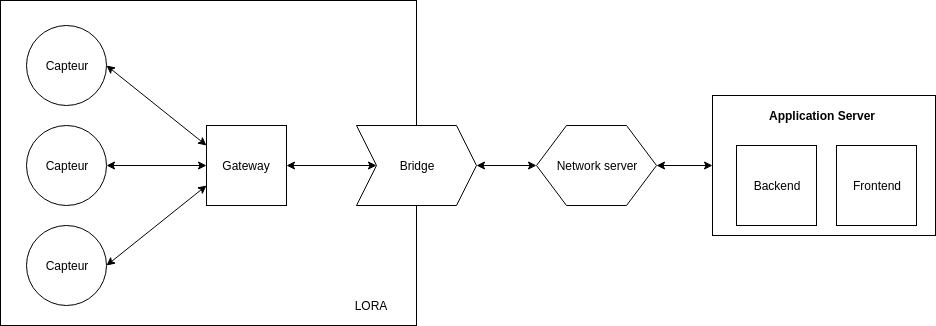
\includegraphics[width=\textwidth]{architecture}
\caption{Schéma de l'architecture du projet}
\end{figure}

\subsection{Exigences de l'application} % Ce qui est nécessaire pour que l'appli fonctionne + au niveau sécu

Pour la sécurité, nous avons interprété les exigences suivantes :

\begin{itemize}
\item[•] L'accès au backend ainsi que l'accès au frontend ne doit être possible que pour les personnes autorisées et authentifiées à l'aide d'un compte soit utilisateur, soit administrateur.
\item[•] Un utilisateur classique ne doit pas pouvoir accéder aux fonctionnalités réservées aux administrateurs.
\item[•] Les données transmises par les capteurs ne doivent pas être lisibles sur le réseau.
\end{itemize}

\newpage
\subsection{Éléments du systèmes}\label{elementssysteme} % Les différents capteurs, gateways, etc...

Afin de rendre ce système fonctionnel, plusieurs composants hardware ainsi que software doivent être utilisés. Les sous-sections suivantes représentent les différents modules hardware utilisés ainsi que les parties software développées pour ce projet.

\subsubsection{Capteurs}
La carte STM32 Nucleo (\autoref{nucleo}) offre aux utilisateurs un moyen abordable et flexible d'essayer de nouveaux concepts et de construire des prototypes avec le microcontrôleur STM32, en choisissant parmi les différentes combinaisons de performances, de consommation d'énergie et de fonctionnalités. Pour les cartes compatibles, le SMPS réduit considérablement la consommation d'énergie en mode Run.

Cette carte sera utilisée comme base pour tous les capteurs déployés dans le terrain.

\begin{figure}[!h]
	\centering
	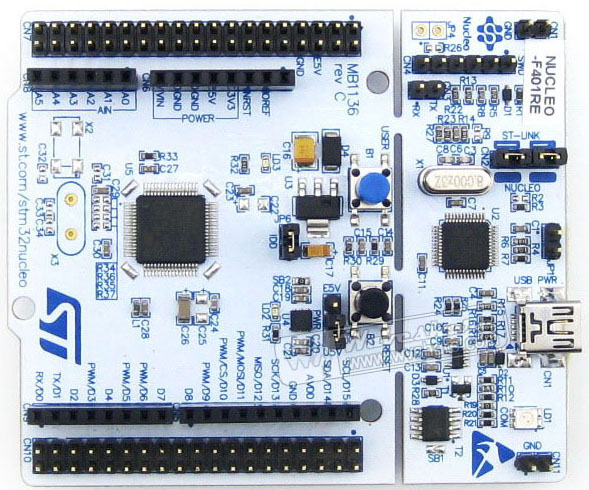
\includegraphics[width=350px]{nucleo}
	\caption{NUCLEO-F401RE}
	\label{nucleo}
\end{figure}

\newpage
Le shield utilisé pour ce projet (\autoref{shield}) rend un Arduino compatible avec plus de 75 capteurs de type clic. C'est un shield simple avec deux prises hôte mikroBUS ™ d'un côté et un connecteur Arduino à l'opposé.

\begin{figure}[!h]
	\centering
	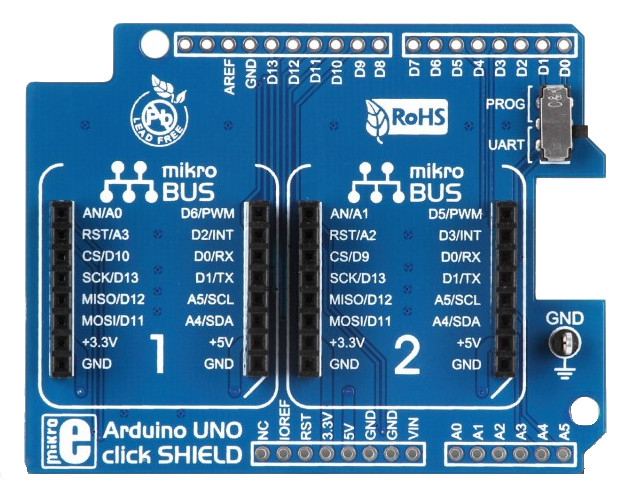
\includegraphics[width=250px]{shield}
	\caption{Arduino Uno Click Shield}
	\label{shield}
\end{figure}

Le module \textit{Environment click} (\autoref{ambient}) mesure la température, l'humidité relative, la pression et les COV (composés organiques volatils gazeux). Le clic intègre le capteur environnemental BME680 de Bosch. Environnement Click est conçu pour fonctionner sur une alimentation de 3,3 V. Il communique avec le microcontrôleur cible via l'interface SPI ou I2C.

\begin{figure}[!h]
	\centering
	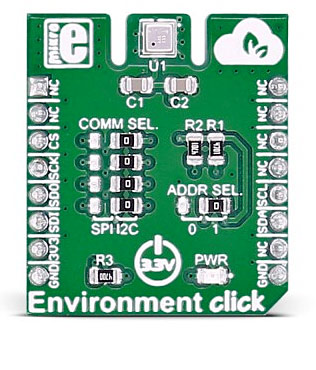
\includegraphics[width=200px]{ambient}
	\caption{Ambient 2 Click BME680}
	\label{ambient}
\end{figure}

\newpage
LoRaWAN ™ ou Low Area Wide Network est une technologie sans fil développée pour permettre des communications à bas débit sur de longues distances, principalement pour les applications IoT et les capteurs.

Le module émetteur-récepteur LoRa longue portée RN2483 de Microchip (\autoref{lora}) est une solution facile à utiliser et à faible consommation d'énergie pour la transmission de données sans fil à longue portée.

Le module RN2483 a une portée spécifiée> 15 km dans les zones rurales et suburbaines, et> 5 km dans les zones urbaines.

Une pile de protocole LoRaWAN ™ classe A est intégrée (périphériques finaux bidirectionnels), ainsi qu'une interface de commande ASCII accessible via UART. La sensibilité élevée du récepteur peut descendre à -148 dBm.
\begin{figure}[!h]
	\centering
	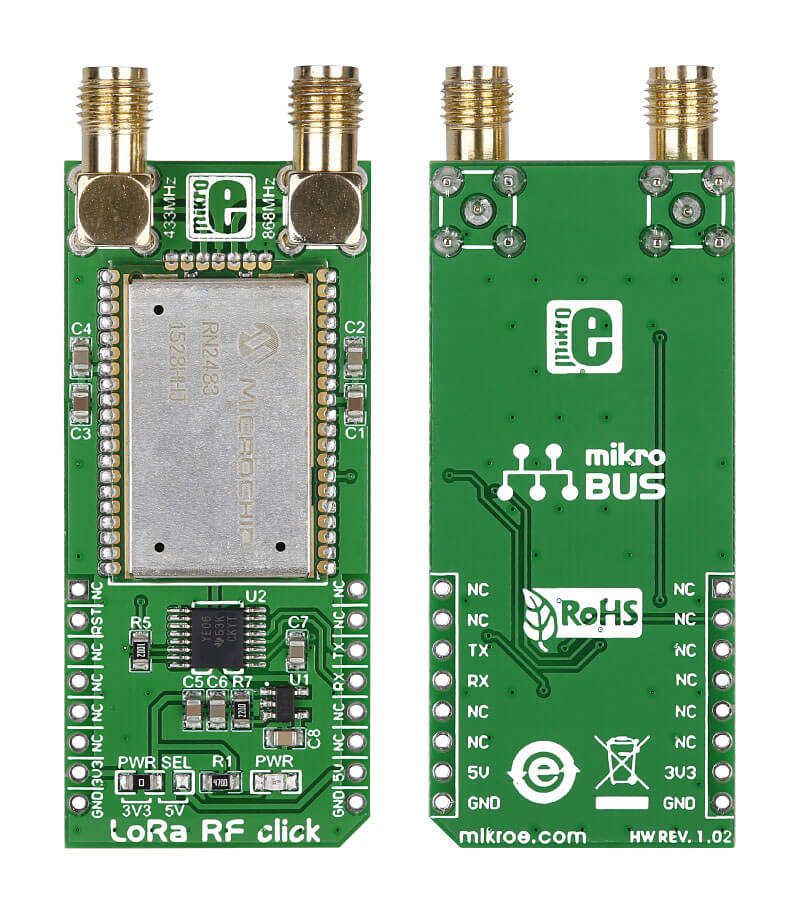
\includegraphics[width=150px]{lora}
	\caption{Lora Click}
	\label{lora}
\end{figure}

Ci-dessous, une photo du montage complet du capteur avec tous les modules attachés :
\begin{figure}[!h]
	\centering
	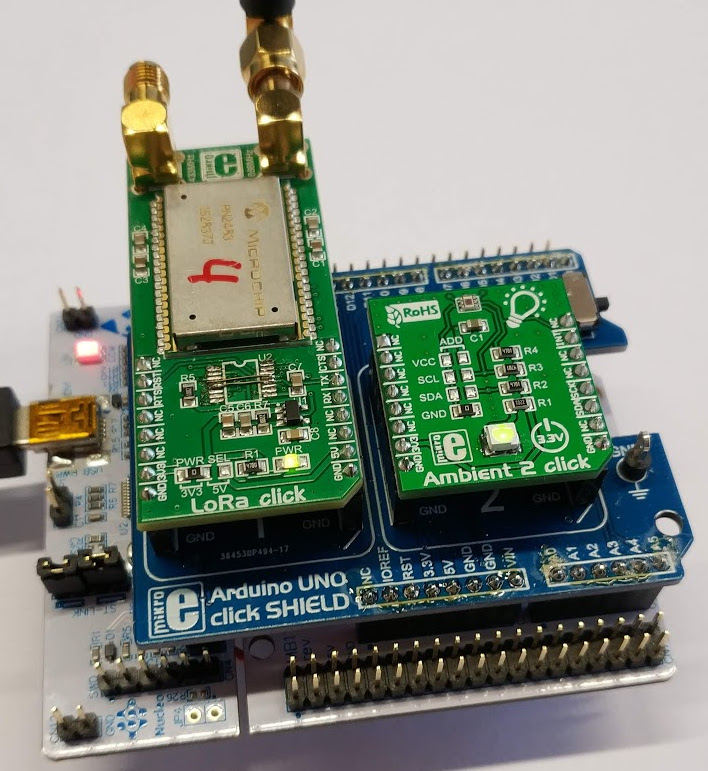
\includegraphics[width=200px]{montage}
	\caption{Montage complet du capteur}
	\label{}
\end{figure}

\newpage
\subsubsection{Gateway}

Le Raspberry Pi 2 Model B est le Raspberry Pi de deuxième génération. Il a remplacé l'original Raspberry Pi 1 Model B+ en février 2015.

Le Raspberry Pi 2 comporte les caractéristiques suivantes :

\begin{itemize}
	\item 900MHz quad-core ARM Cortex-A7 CPU
	\item 1GB RAM
	\item 100 Base Ethernet
	\item 4 Ports USB
	\item 40 pins GPIO
	\item Port HDMI
	\item Jack audio 3.5mm et sortie vidéo composite
	\item Interface Caméra (CSI)
	\item Interface d'affichage (DSI)
	\item Slot pour Micro SD
	\item VideoCore IV 3D coeur graphique
\end{itemize}



\begin{figure}[!h]
	\centering
	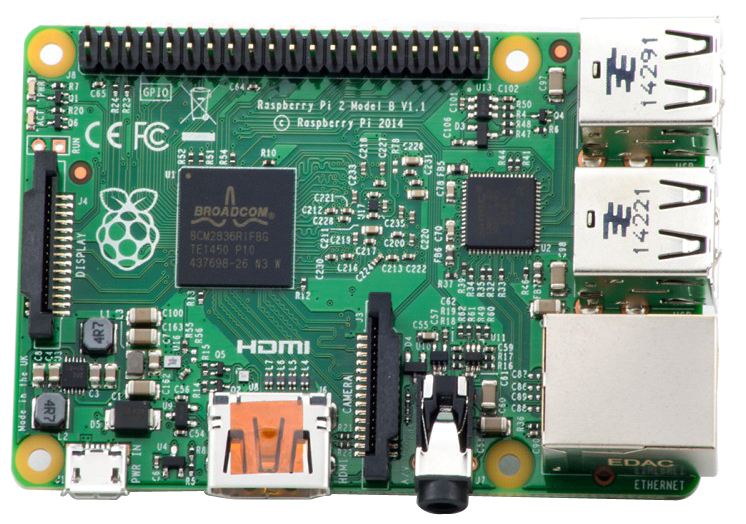
\includegraphics[width=350px]{raspberry}
	\caption{}
	\label{}
\end{figure}

Lora + SHield

\newpage
\subsubsection{Bridge}

Dans notre cas, le bridge fait partie intégrante de la gateway. Sur le schéma dans la \autoref{objectifssysteme}, ce dernier est séparé de la gateway afin de bien représenter le passage de l'utilisation du protocole \textit{LoRa} vers le protocole \textit{MQTT}.

\subsubsection{Network Server}

Ce dernier est divisé en trois parties différentes : Routeur, Broker et Network server.

\subsubsection{Backend}

Le backend est développé en Node.js avec le framework Express. Ce dernier reçoit des informations depuis le network server et traite ces informations avant de pouvoir fournir ces dernières au frontend.

\subsubsection{Frontend}


React
fetch -> update "a la ajax"
mdp local storage

%------------------------ Biens a protéger ---------------------------------
\newpage
\subsection{Biens nécessitants une protections}

Les biens principaux à sécuriser sont toutes les données qui peuvent contenir des informations métier ou clients. Par exemple, les données transmises par les capteurs ne doivent pas être lisibles par des personnes non-autorisées au cours de leur trajet.

Les biens concernés par cette protection sont les suivants :

\begin{itemize}
\item[•] Les données transmises par les capteurs
\begin{itemize}
\item Identité
\item Géo-localisation
\item Données environnementales
\end{itemize}
\item[•] Les données utilisateurs
\begin{itemize}
\item Adresses e-mails \footnote{Afin d'éviter toute réutilisation pour du phishing ou du spamming de masse.}
\item Rôles des utilisateurs \footnote{Pour éviter les vols de session ciblés.}
\item Mots de passe \footnote{Les raisons sont évidentes et de plus ces mots de passe pourraient être ajouté à des listes de brute-force.}
\end{itemize}
\item[•] Le fonctionnement de l'application
\item[•] Les appareils et éléments physiques qui font tourner l'architecture
\end{itemize}

Ces biens doivent être protégés à tous les niveaux et à tous les endroits où elles sont susceptibles d'apparaitre (e.g. des capteurs à la gateway mais aussi de la gateway au serveur d'application).

%------------------------ Périmètre sécurisation ---------------------------
\subsection{Périmètre de sécurisation}

Dans ce projet, la sécurité doit être analysée sur chacun des éléments qui composent l'architecture mais aussi sur les liens entre eux. Il n'y a aucune zone considérée comme "sûre de base", il faut donc penser à tous les éléments suivants :

\begin{itemize}
\item[•] Sécurisation des connexions aux éléments physiques.
\item[•] Sécurisation des trames à l'intérieur du protocole LoRa.
\item[•] Sécurisation des accès au back-end et au front-end.
\item[•] Sécurisation de toutes les communications MQTT.
\item[•] Sécurisation des éléments hébergeant les différents éléments de l'infrastructure.
\item[•] Sécurisation et gestion des version pour les technologies, langages et librairies utilisées.
\end{itemize}

%------------------------ Diagramme des flux -------------------------------
\subsection{Diagramme des flux}

%------------------------ Sources de menaces -------------------------------
\section{Sources de menaces}

Différentes sources de menaces existent autour des applications web mais aussi autour du monde de l'\emph{Internet des objets}. Dans le cadre de notre projet nous retrouvons les catégories de menaces décrites ci-dessous :

\begin{itemize}

\item[•] \textbf{Étudiants kleptomanes}

\begin{tabular}{lp{13cm}}
Motivation: & Gagner un capteur, une gateway, une Raspberry Pi gratuite \\
Cible: & Le matériel \\
Probabilité: & Haute \\
\end{tabular}
\medskip

\item[•] \textbf{Hacker, script-kiddies}

\begin{tabular}{lp{13cm}}
Motivation: & S'amuser, s'entraîner, le faire pour la reconnaissance \\
Cible: & Tout ce qui peut être visé et qui entre dans ses compétences \\
Probabilité: & Moyenne \\
\end{tabular}
\medskip

\item[•] \textbf{Éventuels concurrents}

\begin{tabular}{lp{13cm}}
Motivation: & Récupération des particularités de l'application (espionnage industriel) \\
Cible: & Le fonctionnement de l'application \\
Probabilité: & Moyenne \\
\end{tabular}
\medskip

\item[•] \textbf{Cybercriminels}

\begin{tabular}{lp{13cm}}
Motivation: & Récupérer des adresses mails (spaming) et mots de passe, se servir de l'application web comme passerelle vers son site malveillant ou pour répandre un virus \\
Cible: & Les données des utilisateurs, l'accès à la partie web \\
Probabilité: & Faible \\
\end{tabular}
\medskip

\item[•] \textbf{Organisation étatique}

\begin{tabular}{lp{13cm}}
Motivation: & Récolter des données, espionner \\
Cible: & Toute l'application \\
Probabilité: & Presque nulle \\
\end{tabular}
\medskip

\end{itemize}

%------------------------ Début scénarios ----------------------------------
\newpage
\section{Scénarios d'attaques}
\label{sec:scenarios}

\subsection{Vol d'informations dans la base de données}

\begin{itemize}
\item Injection SQL
\item Conservation des mots de passe dans la DB
\item Accès direct à la base de données (port 3306 ouvert)
\item Gestion version, droits utilisateurs, built-in fonctions
\end{itemize}

\subsection{Contournement d'authentification}

\begin{itemize}
\item XSS
\item Brute-force login
\item CSRF et autres
\item Contrôle d'accès
\item Durée de vie de session
\end{itemize}

\subsection{Récupération passive d'information}

\begin{itemize}
\item SSL/TLS
\item Messages d'erreurs
\end{itemize}

\subsection{Utilisation frauduleuse du matériel}

\begin{itemize}
\item Protection modification du hardware (signature, tamper-proofing)
\item Contrôle d'accès physique
\item Association sécurisée
\end{itemize}

\subsection{Altération des données}

\begin{itemize}
\item Chiffrement des trames LoRa
\item \emph{Man in the middle}
\item Association sécurisée (capteur - serveur)
\end{itemize}

\subsection{Altération du fonctionnement de l'application}

\begin{itemize}
\item Dos
\item Buffer-overflow
\item Trafic jamming
\item Système hébergeur et services pas à jour
\end{itemize}

%------------------------ Contremesures ------------------------------------
\section{Contre-mesures}

%------------------------ Conclusion ---------------------------------------
\section{Conclusion}
\label{sec:conclusion}

%------------------------ Sources ------------------------------------------
\section{Sources}
\label{sec:sources}

\end{document}
